\documentclass[a0paper, portrait]{tikzposter}

\usepackage[colorlinks = true, linkcolor = mb, citecolor = blue, urlcolor = black]{hyperref}

\usepackage{amsmath}
\usepackage{bm}
\usepackage{bbm}
\usepackage{amssymb}
\usepackage{amsthm}
\usepackage{graphicx}
\usepackage{pgfplots}
\usepackage{tikz}
\usepackage{xcolor}

% Tiks libraries.
\pgfplotsset{compat = 1.18}
\usetikzlibrary{fit}

% Colors.
\definecolor{mb}{RGB}{0, 102, 168}
\definecolor{mr}{RGB}{225, 0, 29}
\definecolor{my}{RGB}{255, 255, 0}
\definecolor{bordergray}{RGB}{64, 64, 64}
\definecolor{fillgray}{RGB}{229, 229, 229}

% Title.
\author{Juli\'an Camilo Villaquir\'a\hspace{1in}\textit{Advisor:} Mauricio Junca}
\titlegraphic{\includegraphics[width = 4.5\textwidth]{poster/uniandes.png}}
\settitle{
\centering
\vbox{
\begin{minipage}{0.65\textwidth}
\centering
{\Huge
\textsc{Semidefinite Optimization Approach\\for Calder\'on Inverse Problem}
\par}
\vspace*{1em}
{\huge \@author \par}
\end{minipage}
\begin{minipage}{0.25\textwidth}
\includegraphics[width = \textwidth]{poster/uniandes.png}
\end{minipage}
}}

\definetitlestyle{mytitle}{}{}
\usetitlestyle{mytitle}

% Colors.
\usetheme{Default}

% Background.
\definebackgroundstyle{mybg}{}
\usebackgroundstyle{mybg}

% Title.
\usetitlestyle{Basic}

% My own commands.
\newcommand{\face}{\text{face}}
\renewcommand{\geq}{\geqslant}
\renewcommand{\leq}{\leqslant}
\renewcommand{\phi}{\varphi}
\renewcommand{\epsilon}{\varepsilon}

% Environments.
\newtheorem*{thm}{Theorem}
\newtheorem*{cj}{Conjecture}

\begin{document}
\maketitle
\begin{columns}
\column{0.5}

\block[roundedcorners = 4pt, linewidth = 4pt]{Calder\'on Inverse Problem}
{
\begin{minipage}{0.65\linewidth}
For $\sigma\in L_+^\infty(\Omega)$ let the Neumann-to-Dirichlet operator $\Lambda(\sigma)\in L(L^2(\partial\Omega))$ defined by $\Lambda(\sigma)f=\left.u\right|_{\partial\Omega}$ where $u$ solves
\begin{equation}
\begin{cases}\displaystyle
-\text{div}(\sigma\nabla u) = 0 \text{ in }\Omega,\\
\left.\sigma\frac{\partial u}{\partial n}\right|_{\partial \Omega} = f.
\end{cases}
\label{eq:bvp}
\tag{BVP}
\end{equation}
$\Lambda$ is a decreasing convex differentiable function with compact self-adjoint positive semidefinite values.\\[1em]
Is it possible to invert $\Lambda$? That is, to recover $\sigma$ from the measurement $\Lambda(\sigma)$?
The answer is \textbf{yes}, but it is an extremely ill-posed problem.\\[1em]
Applications include Electrical Impedance Tomography (EIT) and non-destructive material testing.
\end{minipage}
\begin{minipage}{0.35\linewidth}
\begin{tikzfigure}
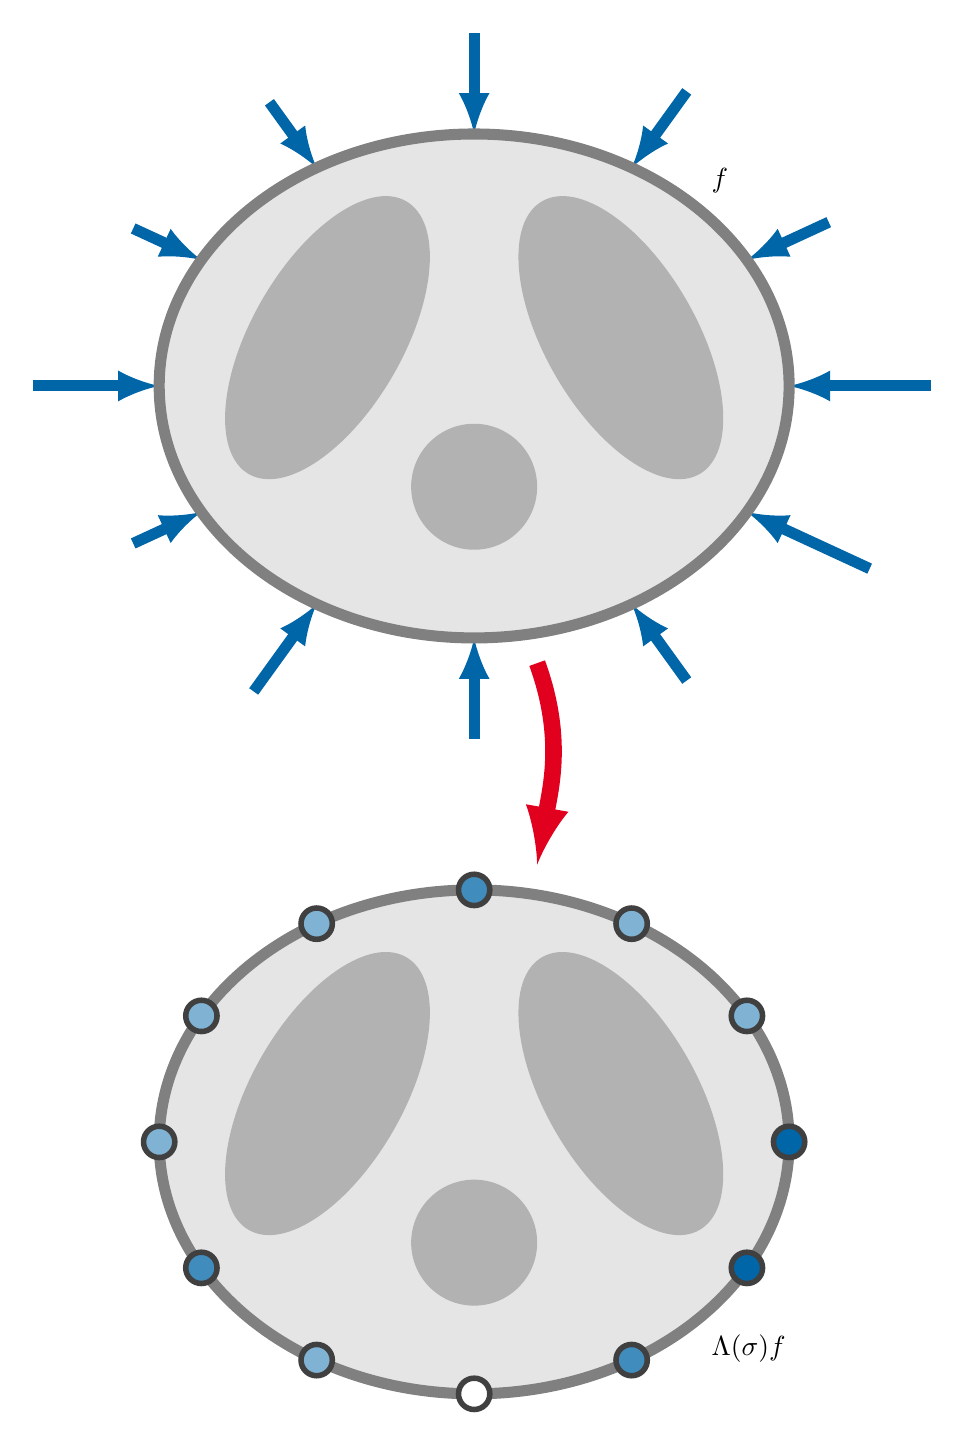
\begin{tikzpicture}[line width = 4pt, scale = 4, x = {(1,0)}, y = {(0,0.8)}, >=latex]
\draw[color = black!50, fill = fillgray] (0,0.0) circle (1.0);
\fill[fill = gray!60] (0,-0.4) ellipse (0.2 and 0.25);
\fill[rotate = 60, fill = gray!60] (-0.1,0.6) ellipse (0.5 and 0.3);
\fill[rotate = -60, fill = gray!60] (0.1,0.6) ellipse (0.5 and 0.3);
\foreach \x in {0,30,...,330}
{
\node[line width = 2pt, circle, inner sep = 4pt, fill = white] at (\x:1.0) {};
\pgfmathrandominteger{\b}{0}{4}
\node[line width = 2pt, circle, inner sep = 4pt, fill = mb, opacity = 0.25 * \b] at (\x:1.0) {};
\node[line width = 2pt, circle, inner sep = 4pt, draw = bordergray] at (\x:1.0) {};
}
\node[anchor = north west] at (-45:1) {$\Lambda(\sigma)f$};
\begin{scope}[shift = {(0,3)}]
\foreach \x in {0,30,...,330}
{
\pgfmathrandominteger{\b}{1}{5}
\draw[<-, mb] (\x:1.0) -- (\x:1.2+0.05*\b);
}
\draw[color = black!50, fill = fillgray] (0,0.0) circle (1.0);
\fill[fill = gray!60] (0,-0.4) ellipse (0.2 and 0.25);
\fill[rotate = 60, fill = gray!60] (-0.1,0.6) ellipse (0.5 and 0.3);
\fill[rotate = -60, fill = gray!60] (0.1,0.6) ellipse (0.5 and 0.3);
\node[anchor = south west] at (45:1) {$f$};
\end{scope}
\draw[line width = 6pt, mr, <-] (0.2,1.1) to[out = 80, in = -70] (0.2,1.9);
\end{tikzpicture}
\end{tikzfigure}
\end{minipage}
}

\block[roundedcorners = 4pt, linewidth = 4pt]{Feasible Set}
{
For two conductivities, $\sigma$ and $\tau$, it is possible to compare $\Lambda(\sigma)$ and $\Lambda(\tau)$ using the Loewner order.
For example, taking into account that
$$\langle\Lambda(\sigma)f,f\rangle = \int_\Omega \sigma \|\nabla u\|^2\,\text dx$$
where $u$ solves \eqref{eq:bvp}, the inequality $\Lambda(\tau)\leq\Lambda(\sigma)$ implies that $\sigma$ dissipates more power into heat than $\tau$ for any boundary condition $f$.
Therefore, for a fixed $\sigma$, natural energy inequalities yield variational constraints which define the \textit{feasible set} $\left\{\tau \in L^\infty_+(\Omega):\Lambda(\tau)\leq \Lambda(\sigma)\right\}$.\\[1em]
By convexity and continuity of $\Lambda$, the feasible set is convex and closed.
$\sigma$ lies in the boundary for if $\eta\neq0$ is non-negative then $\Lambda(\sigma-\eta) \not\leq \Lambda(\sigma)$ by monotonicity and injectivity of $\Lambda$.\\[1em]
Is it possible to characterize $\sigma$ as the optimizer of a functional over the feasible set? 
}

\block[roundedcorners = 4pt, linewidth = 4pt]{Finite-Dimensional Reduction}
{
Suppose that $\Omega$ is divided into pixels $P_1,\dots,P_J$ ordered in such a way that for all $j$ the complement of the set $\bigcup_{k>j}\overline P_k$ is connected and contains a non-empty open subset of $\partial\Omega$.
We identify $\sigma\in\mathbb R^J_+$ with a conductivity given by $\sigma(x)=\sum_{j}\sigma(j)\chi_{P_j}(x)$.\\[1em]
\begin{minipage}{0.7\linewidth}
\begin{thm}
Let $0<a<b$.
Then there exists $c\in\mathbb R^J$ such that for any $\sigma\in[a,b]^J$ the problem
\begin{align*}
& \textup{min}\;\; c\tau \\
& \textup{subject to }\; \tau \in [a,b]^J \\
& \phantom{\textup{subject to }\;} \Lambda(\tau) \leq \Lambda(\sigma)
\end{align*}
has $\sigma$ as its unique optimizer.
\end{thm}
\end{minipage}
\begin{minipage}{0.3\linewidth}
\centering
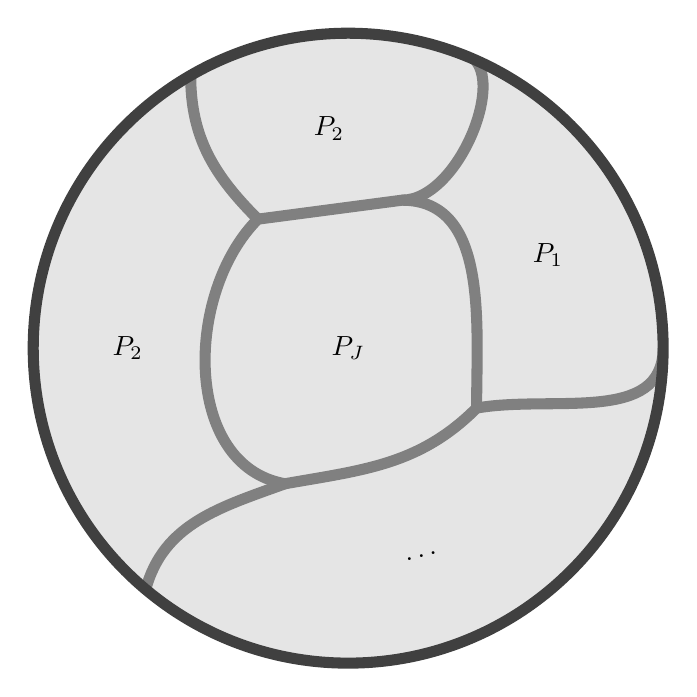
\begin{tikzpicture}[scale = 4, line width = 4pt]
\fill[fill = fillgray] (0,0) circle (1);
\coordinate (A1) at (0:1);
\coordinate (A2) at (70:1);
\coordinate (A3) at (120:1);
\coordinate (A4) at (230:1);
\coordinate (B1) at (-25:0.45);
\coordinate (B2) at (70:0.5);
\coordinate (B3) at (125:0.5);
\coordinate (B4) at (245:0.475);
\begin{scope}
\clip (0,0) circle (1);
\draw[black!50] (A1) to[out = -90, in = 10] (B1);
\draw[black!50] (A2) to[out = 0, in = 0] (B2);
\draw[black!50] (A3) to[out = -90, in = 135] (B3);
\draw[black!50] (A4) to[out = 75, in = 200] (B4);
\draw[black!50] (B1) to[out = 90, in = 0] (B2) to (B3) to[out = 225, in = 170] (B4) to[out = 10, in = -135] (B1);
\end{scope}
\node at (25:0.7) {$P_1$};
\node at (95:0.7) {$P_2$};
\node at (180:0.7) {$P_2$};
\node[rotate = 15] at (290:0.7) {$\dots$};
\node at (0,0) {$P_J$};
\draw[bordergray] (0,0) circle (1);
\end{tikzpicture}
\end{minipage}
}


\block[roundedcorners = 4pt, linewidth = 4pt]{Localized Potentials}
{
Appropriate boundary conditions $f$ can be chosen to study the structure of $K_\sigma := \left\{ \tau\in[a,b]^J : \Lambda(\tau) \leq \Lambda(\sigma) \right\}$.
The localized potentials principle allows, for each $j$, to construct boundary conditions $(f_n)_n$ with high energy in $P_j$ but low energy in $P_{j+1},\dots,P_J$,
$$
\int_{P_j}\sigma\|\nabla u_n\|^2\,\text dx \to \infty
\;\text{ and }\;
\int_{P_k}\sigma\|\nabla u_n\|^2\,\text dx \to 0 \;\text{ for }\; k>j.
$$

\begin{minipage}{0.7\linewidth}
By convexity, we have
\begin{align*}
\langle (\Lambda(\tau) - \Lambda(\sigma))f_n,f_n\rangle &\geq \langle \Lambda'(\sigma)(\tau - \sigma)f_n,f_n\rangle \\
&=\sum_{k} (\tau(k)-\sigma(k))\int_{P_k}\sigma\|\nabla u_n\|^2\,\text dx
\end{align*}
which can be used to discard conductivities $\tau$.
\end{minipage}
\begin{minipage}{0.3\linewidth}
\centering
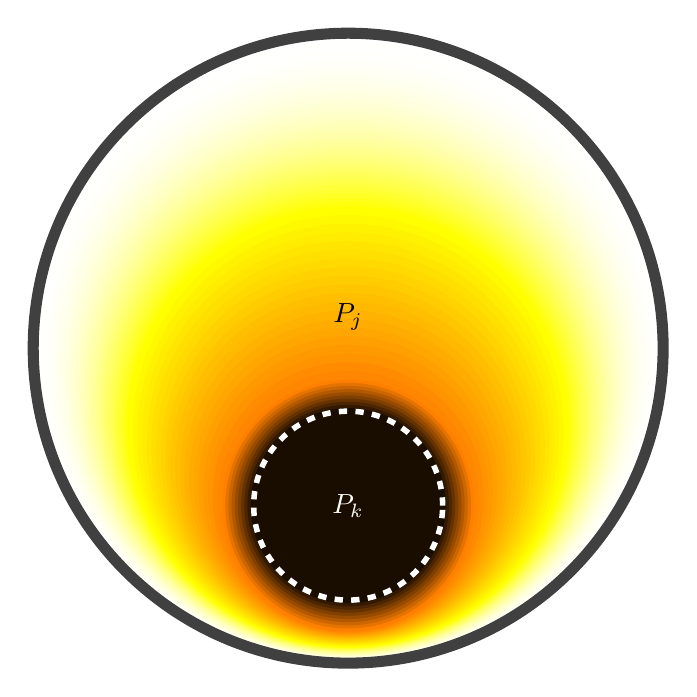
\begin{tikzpicture}[scale = 4, line width = 4pt]
\fill[fill = fillgray] (0,0) circle (1);
\foreach \t in {0,0.025,...,1}
{
\pgfmathsetmacro\k{\t*\t*100}
\fill[fill = my!\k!white] (0,-0.25*\t) circle (1.0 - 0.3 * \t);
}
\foreach \t in {0,0.05,...,1}
{
\pgfmathsetmacro\k{\t*100}
\fill[fill = orange!\k!my] (0,-0.25-0.25*\t) circle (0.7 - 0.3 * \t);
}
\foreach \t in {0,0.1,...,1}
{
\pgfmathsetmacro\k{\t*100}
\fill[fill = black!\k!orange] (0,-0.5) circle (0.4 - 0.1 * \t);
}
\draw[line width = 2pt, dashed, white] (0,-0.5) circle (0.3);
\node at (0,0.1) {$P_j$};
\node[white] at (0,-0.5) {$P_k$};
\draw[bordergray] (0,0) circle (1);
\end{tikzpicture}
\end{minipage}
}

\block[roundedcorners = 4pt, linewidth = 4pt]{}
{
\begin{minipage}{0.3\linewidth}
\centering
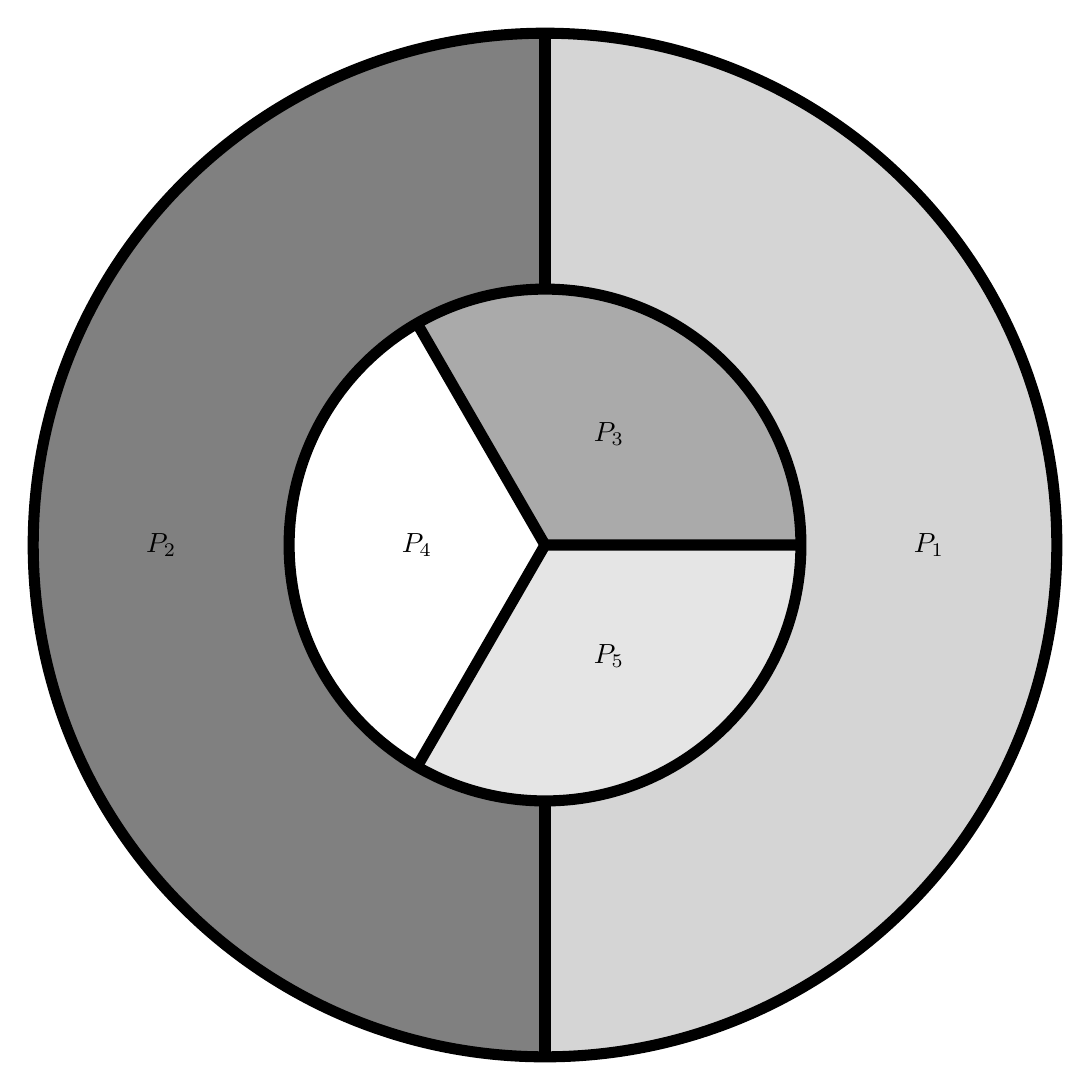
\begin{tikzpicture}[scale = 6.5, line width = 4pt]
\fill[gray!33] (0,1) arc (90:-90:1) -- cycle;
\fill[gray!100] (0,1) arc (90:270:1) -- cycle;
\draw (0,0) circle (1);
\draw (0,-1) -- (0,1);
\fill[gray!67] (0,0) -- (0:0.5) arc (0:120:0.5) -- cycle;
\fill[gray!0] (0,0) -- (120:0.5) arc (120:240:0.5) -- cycle;
\fill[gray!20] (0,0) -- (240:0.5) arc (240:360:0.5) -- cycle;
\draw (0,0) circle (0.5);
\draw (0,0) -- (0:0.5) -- (0,0) -- (120:0.5) -- (0,0) -- (240:0.5) -- cycle;
\node at (0.75,0) {$P_1$};
\node at (-0.75,0) {$P_2$};
\node at (60:0.25) {$P_3$};
\node at (180:0.25) {$P_4$};
\node at (300:0.25) {$P_5$};
\end{tikzpicture}
\end{minipage}
\begin{minipage}{0.7\linewidth}
\raggedleft
\input{poster/normalfanerror}
\end{minipage}
}


\column{0.5}
\block[roundedcorners = 4pt, linewidth = 4pt]{Structure of $\bm{K_\sigma}$}
{
By localized potentials if $\eta$ is any vector such that its first non-zero component is negative then $\tau := \sigma + \eta$ is not feasible.
Therefore, one possible reconstruction algorithm is to start with $\tau = b\mathbbm1$ and decrease one component at a time until $\tau$ is out of $K_\sigma$.
The result can be generalized.\\[1em]
\begin{minipage}{0.7\linewidth}
\begin{thm}
Let $\sigma\in K$ and let $d:\{1,\dots,J\}\to\mathbb N$ defined by $d(j)=1+\textup{dist}(P_j,\partial \Omega)$.
Then, for each $1\leq l \leq \max_j d(j)$, any minimizer $\tau$ of
\begin{align*}
&\textup{min}\;\; \sum_{j\in d^{-1}\left(\{l\}\right)}\tau(j) \\
&\textup{subject to }\; \tau \in K_\sigma \\
&\phantom{\textup{subject to }\;} \tau(k) = \sigma(k) \textup{ if } d(k) < l
\end{align*}
satisfies $\tau(j)=\sigma(j)$ for each $j$ with $d(j)=l$.
\end{thm}
\end{minipage}
\begin{minipage}{0.3\linewidth}
\centering
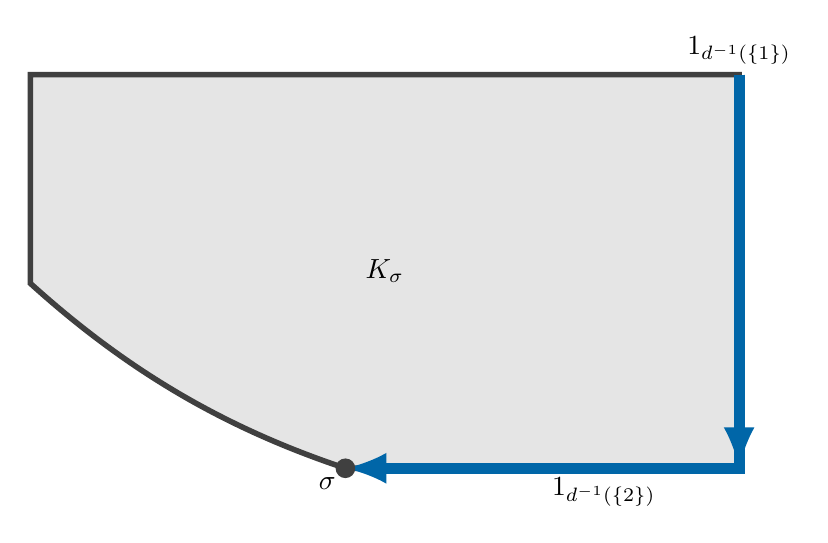
\begin{tikzpicture}[scale = 5, >=latex]
\draw[domain=0.2:1, smooth, variable=\x, bordergray, line width = 2pt, fill = fillgray] plot ({\x}, {
(-(5*\x-5)+sqrt((5*\x-5)^2+36*\x))/6
}) -- (2,1) -- (2,2) -- (0.2,2) -- cycle;
\node at (1.1,1.5) {$K_\sigma$};
\node[anchor = north east] at (1,1) {$\sigma$};
\draw[line width = 4pt, mb, ->] (2,2) -- (2,1);
\draw[line width = 4pt, mb, ->] (2,2) -- (2,1) -- (1,1);
\fill[bordergray] (1,1) circle (0.025);
\node[anchor = south] at (2,2) {$\mathbbm1_{d^{-1}(\{1\})}$};
\node[anchor = north west] at (1.5,1) {$\mathbbm1_{d^{-1}(\{2\})}$};
\end{tikzpicture}
\end{minipage}
}

\block[roundedcorners = 4pt, linewidth = 4pt]{Construction of Weights}
{
\begin{minipage}{0.7\linewidth}
If the functionals $c_1,\dots,c_m$ are defined as $c_l(j)=1$ if $d(j)=l$ and $0$ otherwise then
$$ \face_{c_m}\left(\face_{c_{m-1}}\left(\dots \left(\face_{c_1}\left(K_\sigma\right)\right)\right)\right) = \{\sigma\}.$$
If $K'$ is a polytope and $c_1,\dots,c_m$ are functionals, studying the normal fan to $K'$ yields an $\epsilon>0$ such that 
$$ \face_{c_m}\left(\face_{c_{m-1}}\left(\dots \left(\face_{c_1}\left(K'\right)\right)\right)\right) = \face_{c_1+\epsilon c_2 + \dots + \epsilon^{m-1}c_m}\left(K'\right).$$
\phantom{.}
\vspace{-30pt}
\begin{cj}
There exists an $\epsilon > 0$ such that for each $\sigma\in [a,b]^J$ the unique minimizer of 
\begin{align*}
&\textup{min}\;\; \sum_{j}\epsilon^{d(j)-1}\tau(j) \\
&\textup{subject to }\; \tau \in K \\
&\phantom{\textup{subject to }\;} \Lambda(\tau) \leq \Lambda(\sigma)
\end{align*}
is $\sigma$ $\left(\text{i.e. the weight vector can be chosen as }c = \sum_{l}\epsilon^{l-1} c_l\right)$.
\end{cj}
\end{minipage}
\begin{minipage}{0.3\linewidth}
\centering
\begin{tikzpicture}[scale = 5, >=latex]
\draw[bordergray, line width = 2pt, fill = fillgray] (0.2,1.47) -- (0.2,2) -- (2,2) -- (2,1) -- (1,1) -- cycle;
\node at (1.1,1.5) {$K_\sigma$};
\node[anchor = south] at (2,2) {$c_1$};
\node[anchor = north east] at (2,1) {$c_2$};
\begin{scope}[line width = 2pt]
\fill[mb!15] (1,1) --++ (0,-0.75) arc (-90:-120.43:0.75) -- cycle;
\draw[mb!50, ->] (1,1) --++ (0,-0.6);
\draw[mb!50, ->] (1,0.4) --++ (-0.125,0);
\draw[mb!50, ->] (1,1) --++ (0,-0.6) --++ (-0.125,0);
\draw[mb, ->] (1,1) --++ (-0.125,-0.6);
\node[mb!50, anchor = west] at (1,0.7) {\scriptsize $-c_1$};
\node[mb!50, anchor = north] at (1,0.4) {\scriptsize $-\epsilon c_2$};
\node[mb, anchor = east] at (0.9,0.7) {\small $-c_1-\epsilon c_2$};
\draw[mb!50, dashed] ($(1,1)+(0.6,-0.125)$) --++ (-1.2,0.25);
\end{scope}
\draw[line width = 4pt, mb, ->] (2,2) -- (2,1);
\draw[line width = 4pt, mb, ->] (2,2) -- (2,1) -- (1,1);
\fill[bordergray] (1,1) circle (0.025);
\begin{scope}[line width = 4, shift = {(1.1,3.35)}, scale = 0.9]
\draw[gray, <->] (-1,0) -- (1,0);
\draw[gray, <->] (0,-1) -- (0,1);
\draw[gray, ->] (0,0) -- (-120.43:1);
\fill[mr, opacity = 0.2] (0,-0.6) circle (0.25);
\draw[line width = 2pt, mr, dashed] (0,-0.6) circle (0.25);
\draw[mb, ->] (0,0) -- (0,-0.6);
\draw[mb, ->] (0,0) --++ (0,-0.6) --++ (-0.2,0);
\end{scope}
\end{tikzpicture}
\end{minipage}
}

\block[roundedcorners = 4pt, linewidth = 4pt]{Interior-Point Method}
{
An interior-point method was implemented with barrier function
$$ B(\tau) = -\sum_j\log(b-\tau_j) -\sum_j\log(\tau_j-a) - \log(\det(Y-\hat\Lambda(\tau))) $$
where $\hat\Lambda$ is a finite-dimensional projection of $\Lambda$.
Hessian computation was infeasible, so gradient descent was used.
For simple cases such as when all the $P_j$'s touch the boundary a FreeFEM++ implementation of algorithm converges.
\begin{tikzfigure}
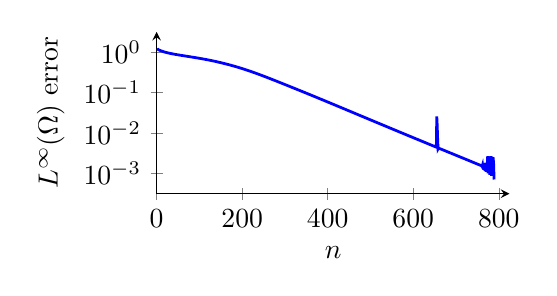
\begin{tikzpicture}
    \begin{axis}[axis lines = left, xmin = 0, xmax = 825, ymax = 0.5, ymin = -3.5, width = .5\linewidth, height = 0.3\linewidth, xlabel = {$n$}, ylabel = {$L^\infty(\Omega)$ error}, legend cell align={left}, legend columns={1}, yticklabels={{$10^0$,$10^{-1}$,$10^{-2}$,$10^{-3}$}}, ytick={{0,-1,-2,-3}}, xtick={{0,200,400,600,800}}]
    \addplot[color=blue, draw opacity={1.0}, line width={1}, solid]
        table[row sep={\\}]
        {
            \\
            1.0  0.08416701454464202  \\
            2.0  0.07228503959816909  \\
            3.0  0.06571620563659901  \\
            4.0  0.059663959379244735  \\
            5.0  0.05402884106966033  \\
            6.0  0.04875073702650333  \\
            7.0  0.04377694611658174  \\
            8.0  0.03907113597795089  \\
            9.0  0.03459459690867442  \\
            10.0  0.03033071094800073  \\
            11.0  0.026249457532898902  \\
            12.0  0.022339922553213674  \\
            13.0  0.018586322169304174  \\
            14.0  0.014972057305417093  \\
            15.0  0.01148821474535504  \\
            16.0  0.008125410435444957  \\
            17.0  0.00486951470336307  \\
            18.0  0.0017188182113785757  \\
            19.0  -0.0013329095502209894  \\
            20.0  -0.004296566287064594  \\
            21.0  -0.007179021766532298  \\
            22.0  -0.009978514896159566  \\
            23.0  -0.01271119581765578  \\
            24.0  -0.015371182823890276  \\
            25.0  -0.017966079927845338  \\
            26.0  -0.02049916933776521  \\
            27.0  -0.02297385203038386  \\
            28.0  -0.025398248932525284  \\
            29.0  -0.027771434681693397  \\
            30.0  -0.03009249144623449  \\
            31.0  -0.03236986784374857  \\
            32.0  -0.03460751136121866  \\
            33.0  -0.036800016231699914  \\
            34.0  -0.0389608888110619  \\
            35.0  -0.04108005180637488  \\
            36.0  -0.043166432836018696  \\
            37.0  -0.04522432708730394  \\
            38.0  -0.04724843808138633  \\
            39.0  -0.04924797464518652  \\
            40.0  -0.05121766575345986  \\
            41.0  -0.05316197021779518  \\
            42.0  -0.055080505556173734  \\
            43.0  -0.056982793884888194  \\
            44.0  -0.05885863689330658  \\
            45.0  -0.06071764357951372  \\
            46.0  -0.06255956206845882  \\
            47.0  -0.06437910328136082  \\
            48.0  -0.06618606773888171  \\
            49.0  -0.06798026599963738  \\
            50.0  -0.06975640836250646  \\
            51.0  -0.07151936241523389  \\
            52.0  -0.07327407844051713  \\
            53.0  -0.07501526534679648  \\
            54.0  -0.07674273127431816  \\
            55.0  -0.07846668982734012  \\
            56.0  -0.08017662455123165  \\
            57.0  -0.08188283013700484  \\
            58.0  -0.08357997126440715  \\
            59.0  -0.08527320009393162  \\
            60.0  -0.08695713899103769  \\
            61.0  -0.0886369800133882  \\
            62.0  -0.09031265005423396  \\
            63.0  -0.09198944295119443  \\
            64.0  -0.09365657018098214  \\
            65.0  -0.09532471275013124  \\
            66.0  -0.09698842797755916  \\
            67.0  -0.09865309061156426  \\
            68.0  -0.10031321558819953  \\
            69.0  -0.10197421849373735  \\
            70.0  -0.10363608502306514  \\
            71.0  -0.1052988006729935  \\
            72.0  -0.1069623507403129  \\
            73.0  -0.10862672031983711  \\
            74.0  -0.11029189430243584  \\
            75.0  -0.11196347748516203  \\
            76.0  -0.11363023573129746  \\
            77.0  -0.11530907897617684  \\
            78.0  -0.11698306616896051  \\
            79.0  -0.11866353071696012  \\
            80.0  -0.1203505229421377  \\
            81.0  -0.1220383416670646  \\
            82.0  -0.12373274544003689  \\
            83.0  -0.12543378584569  \\
            84.0  -0.12714151507718402  \\
            85.0  -0.1288501429257733  \\
            86.0  -0.13056551952236978  \\
            87.0  -0.1322876983909389  \\
            88.0  -0.13402264664193322  \\
            89.0  -0.13575861687616958  \\
            90.0  -0.13750155402151215  \\
            91.0  -0.1392515142235046  \\
            92.0  -0.14100855430914375  \\
            93.0  -0.14277876516934448  \\
            94.0  -0.14455016294362996  \\
            95.0  -0.14633489846243836  \\
            96.0  -0.14812699863699974  \\
            97.0  -0.14992652449929464  \\
            98.0  -0.15173353784313298  \\
            99.0  -0.15355428617708666  \\
            100.0  -0.15538270001563614  \\
            101.0  -0.1572188441766125  \\
            102.0  -0.15906904828152202  \\
            103.0  -0.16092716845938623  \\
            104.0  -0.16279327273898914  \\
            105.0  -0.16467377537007266  \\
            106.0  -0.16656245603398667  \\
            107.0  -0.1684657871579889  \\
            108.0  -0.17037749651824927  \\
            109.0  -0.17229765820099727  \\
            110.0  -0.174232833831479  \\
            111.0  -0.1761766710332937  \\
            112.0  -0.17813579279931568  \\
            113.0  -0.18010379231399248  \\
            114.0  -0.1820873553348572  \\
            115.0  -0.18408001951183076  \\
            116.0  -0.18608186874745977  \\
            117.0  -0.1881063822239325  \\
            118.0  -0.1901336488717284  \\
            119.0  -0.19217718328296124  \\
            120.0  -0.19423037884286753  \\
            121.0  -0.19630015199540077  \\
            122.0  -0.19838669411531834  \\
            123.0  -0.20048330931828925  \\
            124.0  -0.20259009533483524  \\
            125.0  -0.2047141094932114  \\
            126.0  -0.20684856269257454  \\
            127.0  -0.20900058523583767  \\
            128.0  -0.21116332463993506  \\
            129.0  -0.2133439859933134  \\
            130.0  -0.21553565207230782  \\
            131.0  -0.21774560462985934  \\
            132.0  -0.21996686030201365  \\
            133.0  -0.22219953530618916  \\
            134.0  -0.2244510293433215  \\
            135.0  -0.2267142565575078  \\
            136.0  -0.2289966981768051  \\
            137.0  -0.2312911986078428  \\
            138.0  -0.23359788594821054  \\
            139.0  -0.2359243669611832  \\
            140.0  -0.23826337789992777  \\
            141.0  -0.24062261239744268  \\
            142.0  -0.2429947330886301  \\
            143.0  -0.24642799597432183  \\
            144.0  -0.2488013193018576  \\
            145.0  -0.2511954278030447  \\
            146.0  -0.25361059472495123  \\
            147.0  -0.25603143679837026  \\
            148.0  -0.2584737238580849  \\
            149.0  -0.26093774287993693  \\
            150.0  -0.26341582160052446  \\
            151.0  -0.26590812139042136  \\
            152.0  -0.2684148064144475  \\
            153.0  -0.27094414816260415  \\
            154.0  -0.2734883071977065  \\
            155.0  -0.2760474581473086  \\
            156.0  -0.2786300279136114  \\
            157.0  -0.2812197484072088  \\
            158.0  -0.2838333528193568  \\
            159.0  -0.28646278130258623  \\
            160.0  -0.28910822663840025  \\
            161.0  -0.2917698851528327  \\
            162.0  -0.2944479568038772  \\
            163.0  -0.2971512538464993  \\
            164.0  -0.29986282054233476  \\
            165.0  -0.30260014089764076  \\
            166.0  -0.3053460511081211  \\
            167.0  -0.3081094333920082  \\
            168.0  -0.3108993969682576  \\
            169.0  -0.3136984564941002  \\
            170.0  -0.3165156732501159  \\
            171.0  -0.319351284343649  \\
            172.0  -0.3222055315570066  \\
            173.0  -0.32507866147117115  \\
            174.0  -0.32797092559363406  \\
            175.0  -0.33087327665036864  \\
            176.0  -0.3338045210741998  \\
            177.0  -0.33674625376007367  \\
            178.0  -0.33969855366678464  \\
            179.0  -0.3426806205705948  \\
            180.0  -0.34567367900389717  \\
            181.0  -0.34868750814244054  \\
            182.0  -0.35171263711486184  \\
            183.0  -0.35475898587199667  \\
            184.0  -0.35782685421061505  \\
            185.0  -0.3609065783096407  \\
            186.0  -0.3640082978081061  \\
            187.0  -0.367122215414522  \\
            188.0  -0.3702586213374481  \\
            189.0  -0.3734075815833608  \\
            190.0  -0.37657954101217606  \\
            191.0  -0.3797644255829696  \\
            192.0  -0.38297283905668184  \\
            193.0  -0.3861913935939235  \\
            194.0  -0.3894286556711824  \\
            195.0  -0.39268379377191603  \\
            196.0  -0.3959559486785843  \\
            197.0  -0.39924532154217174  \\
            198.0  -0.4025521172143197  \\
            199.0  -0.40587433282507307  \\
            200.0  -0.40921435826176383  \\
            201.0  -0.4125712864271216  \\
            202.0  -0.4159441792547637  \\
            203.0  -0.41933434780689766  \\
            204.0  -0.42274084286617336  \\
            205.0  -0.4261638411062466  \\
            206.0  -0.4296035222243304  \\
            207.0  -0.4330588918293567  \\
            208.0  -0.4365301075299687  \\
            209.0  -0.44001732944677635  \\
            210.0  -0.44352192615168246  \\
            211.0  -0.4470404453030462  \\
            212.0  -0.4505754469138799  \\
            213.0  -0.45412710133504014  \\
            214.0  -0.4576930899372084  \\
            215.0  -0.46127478299382996  \\
            216.0  -0.464871060607384  \\
            217.0  -0.4684833171667079  \\
            218.0  -0.4721104154227816  \\
            219.0  -0.47575117696457864  \\
            220.0  -0.47940831018570235  \\
            221.0  -0.4830793295444404  \\
            222.0  -0.4867643260273238  \\
            223.0  -0.4904633912830103  \\
            224.0  -0.49417661762293313  \\
            225.0  -0.49790409802170876  \\
            226.0  -0.5016445475449876  \\
            227.0  -0.5053994151204008  \\
            228.0  -0.509167392599276  \\
            229.0  -0.5129485383350445  \\
            230.0  -0.5167429104128661  \\
            231.0  -0.5205505666240163  \\
            232.0  -0.5243701118087979  \\
            233.0  -0.5282030299610916  \\
            234.0  -0.5320478988071726  \\
            235.0  -0.5359032428907976  \\
            236.0  -0.5397720471584191  \\
            237.0  -0.5436528464455771  \\
            238.0  -0.54754412034066  \\
            239.0  -0.5514473836640781  \\
            240.0  -0.5553626445014473  \\
            241.0  -0.5592867607191596  \\
            242.0  -0.5632228280226832  \\
            243.0  -0.567169244992644  \\
            244.0  -0.5711259673040563  \\
            245.0  -0.5750929475543152  \\
            246.0  -0.5790701351661554  \\
            247.0  -0.5830558134844197  \\
            248.0  -0.5870515573394652  \\
            249.0  -0.5910573054780267  \\
            250.0  -0.5950712835987827  \\
            251.0  -0.5990933754061343  \\
            252.0  -0.6031252011203676  \\
            253.0  -0.6071649255611596  \\
            254.0  -0.6112124177990292  \\
            255.0  -0.6152693323932054  \\
            256.0  -0.6193319627841098  \\
            257.0  -0.6234037604635567  \\
            258.0  -0.627482782030475  \\
            259.0  -0.6315688689809126  \\
            260.0  -0.6356618567273553  \\
            261.0  -0.6397615744383215  \\
            262.0  -0.643867844874872  \\
            263.0  -0.6479804842240491  \\
            264.0  -0.6520993019292485  \\
            265.0  -0.6562241005175471  \\
            266.0  -0.6603546754240027  \\
            267.0  -0.6644908148129588  \\
            268.0  -0.6686322993963884  \\
            269.0  -0.6727789022493195  \\
            270.0  -0.6769303886223951  \\
            271.0  -0.6810865157516265  \\
            272.0  -0.6852491366007818  \\
            273.0  -0.6894138041969267  \\
            274.0  -0.693584479146565  \\
            275.0  -0.697758781382808  \\
            276.0  -0.7019386121336623  \\
            277.0  -0.7061215330067641  \\
            278.0  -0.7103072409042566  \\
            279.0  -0.7144976736163813  \\
            280.0  -0.7186925740842547  \\
            281.0  -0.7228893821376985  \\
            282.0  -0.7270900729658226  \\
            283.0  -0.7312920228803619  \\
            284.0  -0.7354995938707332  \\
            285.0  -0.7397077809181393  \\
            286.0  -0.7439210178102813  \\
            287.0  -0.7481366195557542  \\
            288.0  -0.7523542529993643  \\
            289.0  -0.7565735745854701  \\
            290.0  -0.7607967338208701  \\
            291.0  -0.7650209109211169  \\
            292.0  -0.7692482834015703  \\
            293.0  -0.7734759616394413  \\
            294.0  -0.7777087543691098  \\
            295.0  -0.781941148088015  \\
            296.0  -0.7861753774197482  \\
            297.0  -0.7904137688041388  \\
            298.0  -0.7946533295667342  \\
            299.0  -0.7988936844832203  \\
            300.0  -0.8031344469512962  \\
            301.0  -0.8073780059134866  \\
            302.0  -0.8116240334130482  \\
            303.0  -0.8158721910595635  \\
            304.0  -0.8201192596470671  \\
            305.0  -0.8243705913000668  \\
            306.0  -0.8286229727427596  \\
            307.0  -0.8328760215436498  \\
            308.0  -0.8371293436786706  \\
            309.0  -0.8413855474709178  \\
            310.0  -0.8456443040516983  \\
            311.0  -0.8499022001477545  \\
            312.0  -0.8541618988946257  \\
            313.0  -0.8584230382468807  \\
            314.0  -0.8626852449385563  \\
            315.0  -0.8669513311840853  \\
            316.0  -0.8712145382314586  \\
            317.0  -0.8754808837902902  \\
            318.0  -0.8797500438946978  \\
            319.0  -0.8840183590170925  \\
            320.0  -0.8882887433855059  \\
            321.0  -0.8925608399196158  \\
            322.0  -0.896834280363229  \\
            323.0  -0.901108685045919  \\
            324.0  -0.9053871554114535  \\
            325.0  -0.9096623372585699  \\
            326.0  -0.9139408360317033  \\
            327.0  -0.9182223297892309  \\
            328.0  -0.9225028529093683  \\
            329.0  -0.9267856234019283  \\
            330.0  -0.9310702860424189  \\
            331.0  -0.9353564744027741  \\
            332.0  -0.9396400311804871  \\
            333.0  -0.9439319051026841  \\
            334.0  -0.9482203563889176  \\
            335.0  -0.9525126438955449  \\
            336.0  -0.9568045257311493  \\
            337.0  -0.9610995351045678  \\
            338.0  -0.9653933295130392  \\
            339.0  -0.9696894965464733  \\
            340.0  -0.9739876809684396  \\
            341.0  -0.9782875162670991  \\
            342.0  -0.9825927967052762  \\
            343.0  -0.9868906155983874  \\
            344.0  -0.9911973438019261  \\
            345.0  -0.9955042239472394  \\
            346.0  -0.999810830704933  \\
            347.0  -1.0041211103147578  \\
            348.0  -1.0084303147390168  \\
            349.0  -1.012746925389585  \\
            350.0  -1.017057182630008  \\
            351.0  -1.0213741494060549  \\
            352.0  -1.0256929881960462  \\
            353.0  -1.0300133221616854  \\
            354.0  -1.0343300624123155  \\
            355.0  -1.0386521615587465  \\
            356.0  -1.0429793474899667  \\
            357.0  -1.0473016530167107  \\
            358.0  -1.0516331690764031  \\
            359.0  -1.0559589172326824  \\
            360.0  -1.0602882661615036  \\
            361.0  -1.0646208884557573  \\
            362.0  -1.0689564458492118  \\
            363.0  -1.0732894476256534  \\
            364.0  -1.077629764085835  \\
            365.0  -1.081966687533454  \\
            366.0  -1.0863049734534669  \\
            367.0  -1.0906495748077962  \\
            368.0  -1.0949894330407741  \\
            369.0  -1.09933488190963  \\
            370.0  -1.1036801361337432  \\
            371.0  -1.1080303176558468  \\
            372.0  -1.1123795081308352  \\
            373.0  -1.1167329167283637  \\
            374.0  -1.121084488677708  \\
            375.0  -1.125439521660219  \\
            376.0  -1.129791821097959  \\
            377.0  -1.1341526891860385  \\
            378.0  -1.1385099926291369  \\
            379.0  -1.1428692118629447  \\
            380.0  -1.147229959588869  \\
            381.0  -1.1515979933567122  \\
            382.0  -1.155960648890933  \\
            383.0  -1.1603235968272185  \\
            384.0  -1.1646927447152422  \\
            385.0  -1.169061423725052  \\
            386.0  -1.1734356453612929  \\
            387.0  -1.177802048689257  \\
            388.0  -1.1821797649403953  \\
            389.0  -1.186555343071081  \\
            390.0  -1.1909282665444676  \\
            391.0  -1.1953048128853998  \\
            392.0  -1.1996846420617966  \\
            393.0  -1.2040674026604314  \\
            394.0  -1.2084457132959319  \\
            395.0  -1.212826074912069  \\
            396.0  -1.2172152594676369  \\
            397.0  -1.2215986150023042  \\
            398.0  -1.2259243605509764  \\
            399.0  -1.230323148553307  \\
            400.0  -1.2347222079538118  \\
            401.0  -1.239113557013422  \\
            402.0  -1.2435117190531577  \\
            403.0  -1.2479087603119006  \\
            404.0  -1.2523041885970174  \\
            405.0  -1.2567053401253845  \\
            406.0  -1.261104009594051  \\
            407.0  -1.2654996622907344  \\
            408.0  -1.2698998330202893  \\
            409.0  -1.2742960351903556  \\
            410.0  -1.2786959394956394  \\
            411.0  -1.283099201652292  \\
            412.0  -1.2875054657764755  \\
            413.0  -1.2919058587185854  \\
            414.0  -1.296308332481705  \\
            415.0  -1.3007124919797564  \\
            416.0  -1.3051179294171318  \\
            417.0  -1.3095242240108365  \\
            418.0  -1.3139309417114848  \\
            419.0  -1.3183376349235292  \\
            420.0  -1.3227438422250801  \\
            421.0  -1.3271490880877796  \\
            422.0  -1.3315622010079495  \\
            423.0  -1.3359735480575947  \\
            424.0  -1.3403826124665108  \\
            425.0  -1.3447984690161436  \\
            426.0  -1.3492111594118525  \\
            427.0  -1.3536201231035392  \\
            428.0  -1.3580346875458975  \\
            429.0  -1.3624445576210398  \\
            430.0  -1.3668592338438292  \\
            431.0  -1.3712784018475008  \\
            432.0  -1.3756914209753848  \\
            433.0  -1.3801080587112688  \\
            434.0  -1.3845279633465768  \\
            435.0  -1.3889401365074217  \\
            436.0  -1.3933653632014877  \\
            437.0  -1.3977818747143378  \\
            438.0  -1.4021999015548627  \\
            439.0  -1.4066190264334115  \\
            440.0  -1.4110388187899068  \\
            441.0  -1.4154588345102166  \\
            442.0  -1.4198786156419227  \\
            443.0  -1.424297690109868  \\
            444.0  -1.428715571431947  \\
            445.0  -1.4331435323793527  \\
            446.0  -1.437569523742742  \\
            447.0  -1.4419810012867456  \\
            448.0  -1.4464134704869163  \\
            449.0  -1.4508303230951078  \\
            450.0  -1.4552553889387856  \\
            451.0  -1.4596759404358528  \\
            452.0  -1.464104016495902  \\
            453.0  -1.4685266096751417  \\
            454.0  -1.4729430841977311  \\
            455.0  -1.4773658227505229  \\
            456.0  -1.4817945539137642  \\
            457.0  -1.4862156914499656  \\
            458.0  -1.4906419752767277  \\
            459.0  -1.4950730983030864  \\
            460.0  -1.4994950246751748  \\
            461.0  -1.5039208615974806  \\
            462.0  -1.5083362637573487  \\
            463.0  -1.51276873041352  \\
            464.0  -1.517189746177003  \\
            465.0  -1.5216129248843466  \\
            466.0  -1.5260378677594082  \\
            467.0  -1.5304641631157254  \\
            468.0  -1.5348913860721738  \\
            469.0  -1.5393190982674045  \\
            470.0  -1.543731658769875  \\
            471.0  -1.548112793334661  \\
            472.0  -1.5525540752452838  \\
            473.0  -1.5569942641730479  \\
            474.0  -1.561417034670624  \\
            475.0  -1.5658533439511306  \\
            476.0  -1.570270850787456  \\
            477.0  -1.5747011296692224  \\
            478.0  -1.5791276307624682  \\
            479.0  -1.5835497698366048  \\
            480.0  -1.5879669460433854  \\
            481.0  -1.5923955307852453  \\
            482.0  -1.5968182471436458  \\
            483.0  -1.6012517864751599  \\
            484.0  -1.6056609819344403  \\
            485.0  -1.6100977048514007  \\
            486.0  -1.6145087076330413  \\
            487.0  -1.6189288506662793  \\
            488.0  -1.6233579524126045  \\
            489.0  -1.6277773914950848  \\
            490.0  -1.6322050237138117  \\
            491.0  -1.6366218250654028  \\
            492.0  -1.6410459991035948  \\
            493.0  -1.6454581105962072  \\
            494.0  -1.6498767171702033  \\
            495.0  -1.6543015556931846  \\
            496.0  -1.6587125603975885  \\
            497.0  -1.663148830513555  \\
            498.0  -1.6675500803618213  \\
            499.0  -1.6719759840369022  \\
            500.0  -1.6763856094870189  \\
            501.0  -1.6808196414954637  \\
            502.0  -1.6852362902370823  \\
            503.0  -1.689655806863066  \\
            504.0  -1.6940563445987942  \\
            505.0  -1.6984802373080135  \\
            506.0  -1.7029058306401959  \\
            507.0  -1.7073105743907209  \\
            508.0  -1.7117380873174486  \\
            509.0  -1.716143425742936  \\
            510.0  -1.7205482645971926  \\
            511.0  -1.7249751824547328  \\
            512.0  -1.7293778161378353  \\
            513.0  -1.7338020100177678  \\
            514.0  -1.738224197443698  \\
            515.0  -1.7426198392873828  \\
            516.0  -1.747036169456117  \\
            517.0  -1.7514488606201986  \\
            518.0  -1.7558573375946487  \\
            519.0  -1.7602610088498403  \\
            520.0  -1.7646845275748064  \\
            521.0  -1.7691025224928822  \\
            522.0  -1.7734885780278766  \\
            523.0  -1.7779193818135268  \\
            524.0  -1.7823169227397662  \\
            525.0  -1.7867328692840903  \\
            526.0  -1.7911404783275664  \\
            527.0  -1.7955390311748998  \\
            528.0  -1.7999551887852472  \\
            529.0  -1.804361353237051  \\
            530.0  -1.8087567552115986  \\
            531.0  -1.8131688506588615  \\
            532.0  -1.8175691594777919  \\
            533.0  -1.8219856833492611  \\
            534.0  -1.8263893410227663  \\
            535.0  -1.8307792754140484  \\
            536.0  -1.8351843221126358  \\
            537.0  -1.8395744704346513  \\
            538.0  -1.8439791275369752  \\
            539.0  -1.8483982816208278  \\
            540.0  -1.8528009717073004  \\
            541.0  -1.857186230013395  \\
            542.0  -1.8615846422123694  \\
            543.0  -1.865996156026674  \\
            544.0  -1.8703884899595722  \\
            545.0  -1.8747931477969726  \\
            546.0  -1.8791771667496322  \\
            547.0  -1.883572674185739  \\
            548.0  -1.8879795671250104  \\
            549.0  -1.8923638394563085  \\
            550.0  -1.896758581403767  \\
            551.0  -1.9011636587599476  \\
            552.0  -1.9055789306936546  \\
            553.0  -1.9099689498524506  \\
            554.0  -1.9143681394973553  \\
            555.0  -1.91874030436246  \\
            556.0  -1.9231205479955094  \\
            557.0  -1.9275454207628202  \\
            558.0  -1.9319044464597044  \\
            559.0  -1.936307667785302  \\
            560.0  -1.940718100398546  \\
            561.0  -1.9450972318097581  \\
            562.0  -1.949482307432866  \\
            563.0  -1.9538730561891156  \\
            564.0  -1.9582691971193615  \\
            565.0  -1.962630588533852  \\
            566.0  -1.9670362238053838  \\
            567.0  -1.9714056779495819  \\
            568.0  -1.9758195405199606  \\
            569.0  -1.9801957285483558  \\
            570.0  -1.9845745466869105  \\
            571.0  -1.988955623768887  \\
            572.0  -1.9933385765623792  \\
            573.0  -1.9977230095011371  \\
            574.0  -2.0021085144137802  \\
            575.0  -2.006494670251752  \\
            576.0  -2.0108810428163095  \\
            577.0  -2.0152671844849372  \\
            578.0  -2.0196526339375436  \\
            579.0  -2.0240369158829163  \\
            580.0  -2.0284195407858294  \\
            581.0  -2.032800004595318  \\
            582.0  -2.0371777884746027  \\
            583.0  -2.0415523585332633  \\
            584.0  -2.0459231655621912  \\
            585.0  -2.0502896447719743  \\
            586.0  -2.0547004716503454  \\
            587.0  -2.059057033813084  \\
            588.0  -2.063407482053939  \\
            589.0  -2.0678019512833465  \\
            590.0  -2.0721900553487984  \\
            591.0  -2.076571143533622  \\
            592.0  -2.0809445476352253  \\
            593.0  -2.0853095817306766  \\
            594.0  -2.089665541951845  \\
            595.0  -2.0940656353474107  \\
            596.0  -2.098401804487435  \\
            597.0  -2.102781704662812  \\
            598.0  -2.1071506412809833  \\
            599.0  -2.111507829572791  \\
            600.0  -2.1159091760536715  \\
            601.0  -2.1202982906653087  \\
            602.0  -2.124616474909866  \\
            603.0  -2.1290364773117374  \\
            604.0  -2.133383824937268  \\
            605.0  -2.13777513050761  \\
            606.0  -2.142090798086984  \\
            607.0  -2.146510632638049  \\
            608.0  -2.1508529608651084  \\
            609.0  -2.1552391450760253  \\
            610.0  -2.1596073577243566  \\
            611.0  -2.1639565996504087  \\
            612.0  -2.1682858494988517  \\
            613.0  -2.1726586902267453  \\
            614.0  -2.1770107214519405  \\
            615.0  -2.1814068058695573  \\
            616.0  -2.185781225346454  \\
            617.0  -2.19013286470566  \\
            618.0  -2.194460585292444  \\
            619.0  -2.1988318658128923  \\
            620.0  -2.2031782499420984  \\
            621.0  -2.20756857243498  \\
            622.0  -2.2119329764613656  \\
            623.0  -2.2162702213150465  \\
            624.0  -2.220651219013949  \\
            625.0  -2.225003944977587  \\
            626.0  -2.229400738270985  \\
            627.0  -2.233693707341315  \\
            628.0  -2.238104672691805  \\
            629.0  -2.2424090890207276  \\
            630.0  -2.2468332569165708  \\
            631.0  -2.251148062298157  \\
            632.0  -2.2555061667069425  \\
            633.0  -2.2598294432102777  \\
            634.0  -2.264196189780813  \\
            635.0  -2.268607289478572  \\
            636.0  -2.272900799260318  \\
            637.0  -2.277319415714293  \\
            638.0  -2.2816172952463543  \\
            639.0  -2.28595813307659  \\
            640.0  -2.290342796638692  \\
            641.0  -2.294686572038997  \\
            642.0  -2.299074232807868  \\
            643.0  -2.303419327892391  \\
            644.0  -2.3077201189113254  \\
            645.0  -2.3120639267418706  \\
            646.0  -2.316451620599578  \\
            647.0  -2.3207931839508102  \\
            648.0  -2.3251785877591677  \\
            649.0  -2.329515969460497  \\
            650.0  -2.3338034294358985  \\
            651.0  -2.3382282547792737  \\
            652.0  -2.342507458127509  \\
            653.0  -2.346925775278984  \\
            654.0  -2.3511944726195426  \\
            655.0  -1.5910042697844333  \\
            656.0  -1.8078623641102767  \\
            657.0  -2.1316737157765555  \\
            658.0  -2.3939877993303966  \\
            659.0  -2.3757625399962476  \\
            660.0  -2.377519954408151  \\
            661.0  -2.3816833173815612  \\
            662.0  -2.385992593692387  \\
            663.0  -2.3903450575769014  \\
            664.0  -2.3947415834578325  \\
            665.0  -2.399074201402185  \\
            666.0  -2.403340532324484  \\
            667.0  -2.407427190324092  \\
            668.0  -2.4121131838263  \\
            669.0  -2.4163969049685114  \\
            670.0  -2.4207233004348443  \\
            671.0  -2.425093229028977  \\
            672.0  -2.429390832026711  \\
            673.0  -2.4337313877670557  \\
            674.0  -2.4381157635146344  \\
            675.0  -2.4424245521310084  \\
            676.0  -2.4467765184972334  \\
            677.0  -2.4511725367361623  \\
            678.0  -2.455489532297964  \\
            679.0  -2.459849871076137  \\
            680.0  -2.464127965745995  \\
            681.0  -2.468576353296898  \\
            682.0  -2.4728126956910033  \\
            683.0  -2.477221067795658  \\
            684.0  -2.4815430054298364  \\
            685.0  -2.4859083860755016  \\
            686.0  -2.490183804566544  \\
            687.0  -2.494501731298281  \\
            688.0  -2.498863020040613  \\
            689.0  -2.503268550546344  \\
            690.0  -2.5075794532805835  \\
            691.0  -2.511933576358457  \\
            692.0  -2.5161892197315403  \\
            693.0  -2.520630970718592  \\
            694.0  -2.5249731305731764  \\
            695.0  -2.529212226689521  \\
            696.0  -2.5336414801919553  \\
            697.0  -2.5379664640079063  \\
            698.0  -2.5423349524045373  \\
            699.0  -2.546594912530522  \\
            700.0  -2.5508970725445543  \\
            701.0  -2.555242276897371  \\
            702.0  -2.5596313956432684  \\
            703.0  -2.563906188888902  \\
            704.0  -2.568223477881274  \\
            705.0  -2.572584116012029  \\
            706.0  -2.576988982640247  \\
            707.0  -2.581273353593982  \\
            708.0  -2.585600411884267  \\
            709.0  -2.589971016709555  \\
            710.0  -2.5942154118231047  \\
            711.0  -2.5986740319681125  \\
            712.0  -2.6030047700769776  \\
            713.0  -2.607379129192057  \\
            714.0  -2.611620376333784  \\
            715.0  -2.615903451606663  \\
            716.0  -2.6202291882722015  \\
            717.0  -2.6245984447417623  \\
            718.0  -2.6290121055990574  \\
            719.0  -2.6332843750576544  \\
            720.0  -2.637599089850307  \\
            721.0  -2.641957101842932  \\
            722.0  -2.6463592888066834  \\
            723.0  -2.650612246124837  \\
            724.0  -2.65510350499163  \\
            725.0  -2.659443394119797  \\
            726.0  -2.6636268679632678  \\
            727.0  -2.6680532118567952  \\
            728.0  -2.6723208628525246  \\
            729.0  -2.676837176080194  \\
            730.0  -2.6811924613345495  \\
            731.0  -2.685381356896551  \\
            732.0  -2.6898236192199447  \\
            733.0  -2.6940970125792782  \\
            734.0  -2.698412873718869  \\
            735.0  -2.7027720551838486  \\
            736.0  -2.7071754354522457  \\
            737.0  -2.711623919997646  \\
            738.0  -2.715892608144084  \\
            739.0  -2.7204317579208106  \\
            740.0  -2.7245579556884554  \\
            741.0  -2.7291890727998065  \\
            742.0  -2.733399726404163  \\
            743.0  -2.737889044346037  \\
            744.0  -2.7421853208876152  \\
            745.0  -2.74652452352852  \\
            746.0  -2.7509075187224936  \\
            747.0  -2.7553351994246467  \\
            748.0  -2.7595587577877905  \\
            749.0  -2.7640759880779235  \\
            750.0  -2.768385840156662  \\
            751.0  -2.7727388914084683  \\
            752.0  -2.777136016610204  \\
            753.0  -2.7815781173817826  \\
            754.0  -2.7858008351871812  \\
            755.0  -2.79033292116515  \\
            756.0  -2.794371478056376  \\
            757.0  -2.799267847500519  \\
            758.0  -2.802838764420948  \\
            759.0  -2.8092293741818763  \\
            760.0  -2.8083904640924096  \\
            761.0  -2.8266484024661716  \\
            762.0  -2.7919438401262724  \\
            763.0  -2.884866533126306  \\
            764.0  -2.745073300131943  \\
            765.0  -2.9095418410349363  \\
            766.0  -2.7419455205851584  \\
            767.0  -2.92534175920526  \\
            768.0  -2.7397932554807225  \\
            769.0  -2.9406004379366086  \\
            770.0  -2.736703138330469  \\
            771.0  -2.958778173170083  \\
            772.0  -2.7424252536715055  \\
            773.0  -2.9459359710582094  \\
            774.0  -2.5711223169059476  \\
            775.0  -2.9962951048194872  \\
            776.0  -2.6458869789354162  \\
            777.0  -2.9950052062476185  \\
            778.0  -2.5792872513805722  \\
            779.0  -3.034531439174178  \\
            780.0  -2.5917559897118925  \\
            781.0  -3.0220171170841303  \\
            782.0  -2.5743698934820505  \\
            783.0  -3.0592010527161024  \\
            784.0  -2.7495741802090343  \\
            785.0  -3.053269105736425  \\
            786.0  -2.624582672551342  \\
            787.0  -2.628257467250717  \\
            788.0  -2.77210716809974  \\
            789.0  -3.1495104289104803  \\
        }
        ;
\end{axis}
\end{tikzpicture}

\end{tikzfigure}
}

\block[roundedcorners = 4pt, linewidth = 4pt]{Numerical Instability}{
\begin{minipage}{0.7\linewidth}
There are several factors affecting the behaviour of the algorithm:
\begin{itemize}
\item[\textcolor{mb}{-}] The size of the projection $\hat\Lambda$ changes the shape of $K_\sigma$.
\item[\textcolor{mb}{-}] The choice of $\epsilon$ depends on $\hat\Lambda$ and, in principle, on $\sigma$.
\end{itemize}
\end{minipage}
\begin{minipage}{0.3\linewidth}
\centering
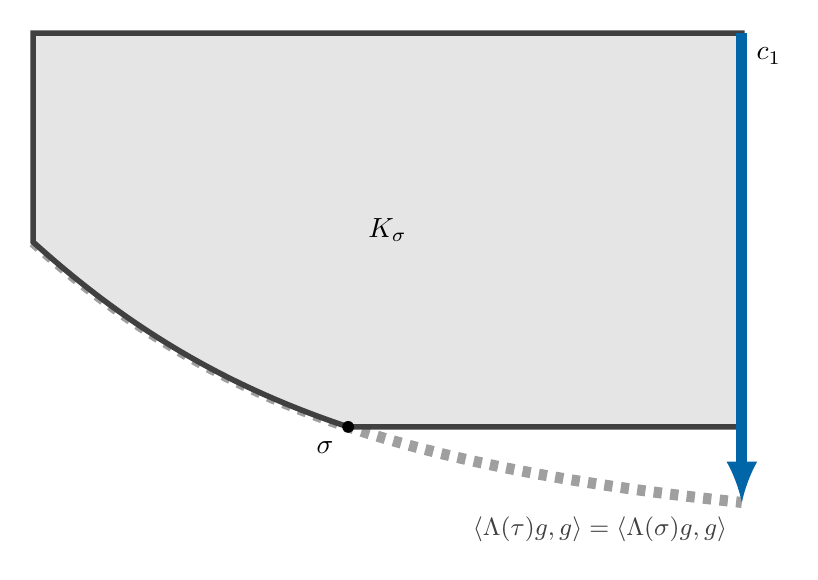
\begin{tikzpicture}[scale = 5, >=latex, line width = 4pt]
\draw[domain=0.2:2, smooth, variable=\x, dashed, gray!75] plot ({\x}, {
(-(5*\x-5)+sqrt((5*\x-5)^2+36*\x))/6
});
\draw[bordergray, line width = 2pt, domain=0.2:1, smooth, variable=\x, fill = fillgray] plot ({\x}, {
(-(5*\x-5)+sqrt((5*\x-5)^2+36*\x))/6
}) -- (2,1) -- (2,2) -- (0.2,2) -- cycle;
\draw[mb, ->] (2,2) -- (2,0.808);
\node at (1.1,1.5) {$K_\sigma$};
\node[anchor = north east, bordergray] at (2,0.808) {\small $ \langle\Lambda(\tau)g,g\rangle = \langle\Lambda(\sigma)g,g\rangle$};
\node[anchor = north west] at (2,2) {$c_1$};
\fill[black] (1,1) circle (0.015);
\node[anchor = north east] at (1,1) {$\sigma$};
\end{tikzpicture}
\end{minipage}
}

\block[roundedcorners = 4pt, linewidth = 4pt]{}
{
\begin{minipage}{0.3\linewidth}
\centering
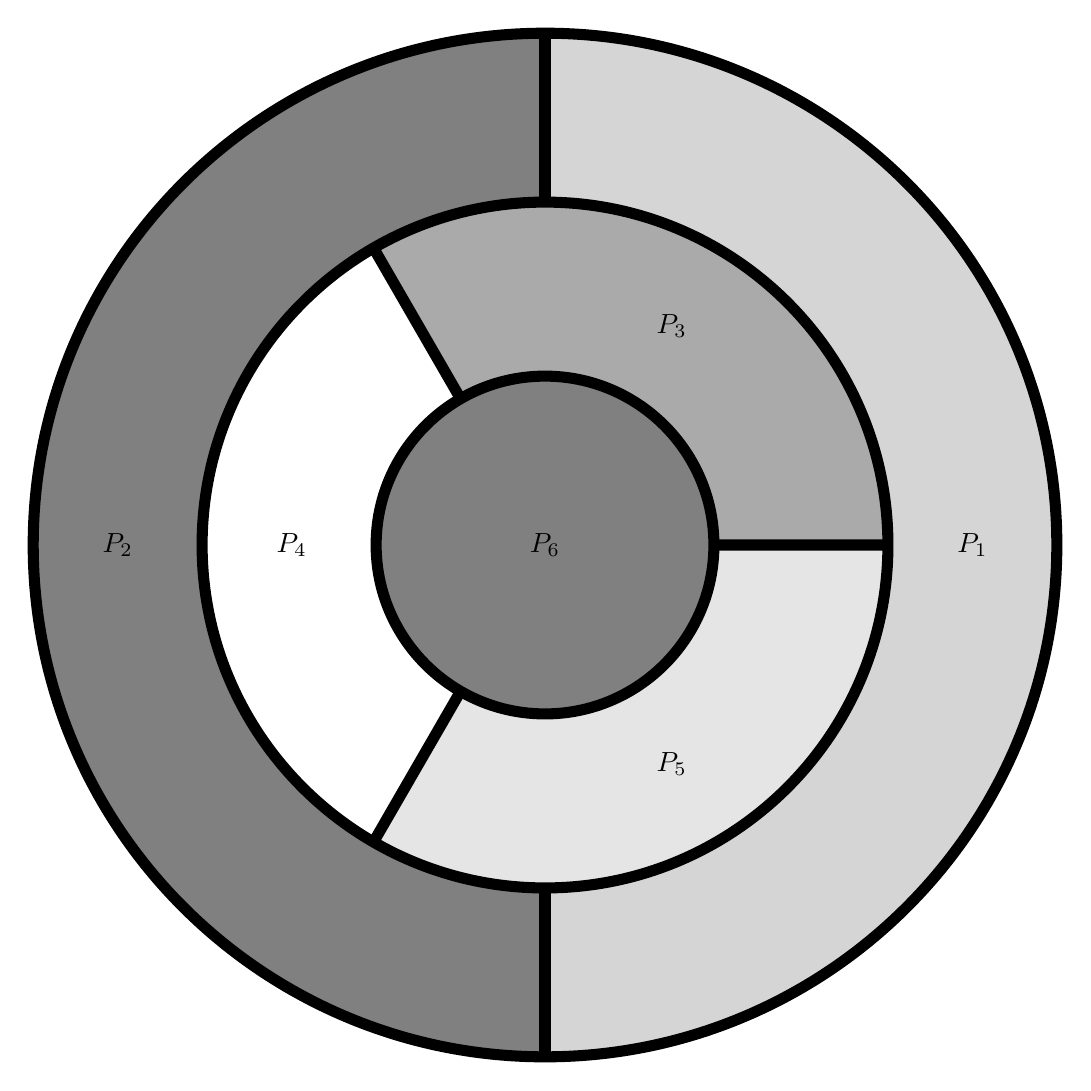
\begin{tikzpicture}[scale = 6.5, line width = 4pt]
\fill[gray!33] (0,1) arc (90:-90:1) -- cycle;
\fill[gray!100] (0,1) arc (90:270:1) -- cycle;
\draw (0,0) circle (1);
\draw (0,-1) -- (0,1);
\fill[gray!67] (0,0) -- (0:0.67) arc (0:120:0.67) -- cycle;
\fill[gray!0] (0,0) -- (120:0.67) arc (120:240:0.67) -- cycle;
\fill[gray!20] (0,0) -- (240:0.67) arc (240:360:0.67) -- cycle;
\draw (0,0) circle (0.67);
\draw (0,0) -- (0:0.67) -- (0,0) -- (120:0.67) -- (0,0) -- (240:0.67) -- cycle;
\fill[gray!100] (0,0) circle (0.33);
\draw (0,0) circle (0.33);
\node at (0.835,0) {$P_1$};
\node at (-0.835,0) {$P_2$};
\node at (60:0.495) {$P_3$};
\node at (180:0.495) {$P_4$};
\node at (300:0.495) {$P_5$};
\node at (0:0) {$P_6$};
\end{tikzpicture}
\end{minipage}
\begin{minipage}{0.7\linewidth}
\raggedleft
\input{poster/coordinatedescent}
\end{minipage}
}

\end{columns}

\end{document}
